% !TeX root = ../../infdesc.tex
\section{Sets}
\secbegin{secSets}
\index{set|(}

Começamos redefinindo a noção de \textit{conjunto} com um nível de precisão maior do que o fornecido em \Cref{chGettingStarted}. Em sua essência, os conjuntos parecem extremamente simples – conjuntos são apenas coleções de objetos – exceto que, se não forem controlados, essa caracterização de um conjunto leva a inconsistências lógicas, como o infame \textit{paradoxo de Russell}.

Esses paradoxos lógicos podem ser superados restringindo-nos a trabalhar dentro de um \textit{universo} $\mathcal{U}$, que consideramos ser um conjunto tão grande que contém todos os objetos matemáticos que queremos falar sobre. Esta é uma questão sutil, que está bem além do escopo desta seção, mas será discutida mais detalhadamente em \Cref{secZFC}.

\begin{definition}
\label{defSet}
\index{set}
\index{element}
\index{universal set}
\index{universe!of discourse}
Um \textbf{conjunto}\index{set} é uma coleção de \textbf{elementos} de um \textbf{universo de discurso}\index{universo de discurso} especificado. A coleção de tudo no universo do discurso é chamada de \textbf{conjunto universal}\index{set!universal}, denotado por $\mathcal{U}$\nindex{U}{$\mathcal{U}$}{conjunto universal} \inlatex{mathcal\{U\}}\lindexmmc{mathcal}{$\mathcal{A}, \mathcal{B}, \dots$}.

A expressão $x \in X$\nindex{in}{$\in$}{element} \inlatex{in}\lindexmmc{in}{$\in$} denota a afirmação de que $x$ é um elemento de $X$; escrevemos $x \not \in X$ \inlatex{not\textbackslash{}in}\lindexmmc{not}{$\not\in, \not\equiv, \dots$} para significar $\neg (x \in X)\neg (x \in X)$, ou seja, $x$ não é um elemento de $X$.
\end{definition}

\begin{example}
Em \Cref{chGettingStarted}, introduzimos cinco conjuntos: o conjunto $\mathbb{N}$ de números naturais, o conjunto $\mathbb{Z}$ de inteiros, o conjunto $\mathbb{Q}$ de números racionais, o conjunto $\mathbb{R}$ de números reais e o conjunto $\mathbb{C}$ de números complexos.
\end{example}

\begin{exercise}
Quais das seguintes proposições são verdadeiras e quais são falsas?
\[ \frac{1}{2} \in \mathbb{Z} \qquad \frac{1}{2} \in \mathbb{Q} \qquad \mathbb{Z} \in \mathbb{Q} \qquad \mathbb{Z} \in \mathcal{U} \qquad \frac{1}{2} \in \mathcal{U} \] 
\hintlabel{exElementsOfSets}{%
Pense no que `$a \in X$' \textit{realmente significa}---não se deixe enganar pela sua intuição.
}
\end{exercise}

Evitaresmos nos referir explicitamente ao conjunto universal $\mathcal{U}$ sempre que possível, mas ele sempre estará lá em segundo plano. Isto é conveniente porque não precisamos mais nos preocupar com o domínio de discursos das variáves livres (como fizemos em \Cref{defPredicate}), para que possamos abreviar `$\forall x \in \mathcal{U},\, p(x)$' por `$\forall x,\, p(x)$', e `$\exists x \in \mathcal{U},\, p(x)$' por `$\exists x,\, p(x)$'.

Observe que sob esta convenção:
\begin{itemize}
\item $\forall x \in X,\, p(x)$ é lógicamente equivalente a $\forall x,\, (x \in X \Rightarrow p(x))$; e
\item $\exists x \in X,\, p(x)$ é logicamente equivalente a  $\exists x,\, (x \in X \wedge p(x))$.
\end{itemize}

\subsection*{Specifying a set}
Uma forma de definir um conjunto é simplesmente descrevê-lo em palavras, como fizemos até agora. Existem outras formas mais concisas de especificar conjuntos, que também eliminam essa ambiguidade do processo.

\textbf{Lists.}\index{list notation}
Uma maneira é simplesmente fornecer uma \textbf{lista} dos elementos do conjunto. Para especificar que a lista denota um conjunto, colocamos a lista entre $\{\{colchetes\}\}$\nindex{set}{$\{ \cdots \$}{set notation} \inlatex{\{,\textbackslach{}\}}\lindexmmc{\{\dots\textbackslash{}\}}{$\{\dots\}$}. Por exemplo, o seguinte é uma especificação de um conjunto XX, cujos elementos são os números naturais entre 00 e 55 (inclusive):
\[ X = \{ 0, 1, 2, 3, 4, 5 \} \]

\textbf{Listas implícitas.}\index{notaçao de listas implícitas}
Às vezes, uma lista pode ser muito longa para ser escrita — talvez até infinita — ou o comprimento da lista pode depender de uma variável. Nestes casos será conveniente usar uma \textbf{lista implícita}, na qual alguns elementos da lista são escritos, e o resto fica implícito escrevendo reticências `$\dots$' \inlatex{pontos} \lindexmmc{pontos}{$\dots$}. Por exemplo, a afirmação
\[ X = \{ 1, 4, 9, \dots, n^2 \} \]
significa que $X$ é o conjunto cujos elementos são todos os números quadrados de $1$ a $n^2$, onde $n$ é algum número. As listas implícitas podem ser ambíguas, pois dependem da capacidade do leitor de inferir o padrão que está sendo seguido, portanto, use-as com cautela!

\textbf{Set-builder notation.}\index{set-builder notation}
Em geral, as listas implícitas podem ser ambíguas, portanto, na prática, elas são evitadas, a menos que a lista implícita seja muito simples, como um conjunto de números consecutivos como $\{3, 4, \dots, 9 \}$. Na verdade, muitos conjuntos nem sequer podem ser listados desta forma.

Para contornar isso, podemos usar \textit{notação set-builder}, que é um meio de especificar um conjunto em termos das propriedades que seus elementos satisfazem. Dado um conjunto $X$, o conjunto de elementos de $X$ que satisfazem alguma propriedade $p(x)$ é denotado
\[ \{ x \in X \mid p(x) \} \]
A barra `$\mid$' \inlatex{mid}\lindexmmc{mid}{$\mid$} separa o nome da variável da fórmula que eles tornam verdadeira --- alguns autores usam dois pontos (como em $\{ x \in X : p(x) \}$).

O conjunto $\{ x \in X \mid p(x) \}$ é lido em voz alta como `o conjunto de $x \in X$ tal que $p(x)$', mas cuidado --- nem a barra `$\mid$' nem os dois pontos `$:$' significam `tal que' em outros contextos.

\begin{example}
\label{exSetsSpecifyUniverses}
O conjunto de todos os inteiros pares pode ser escrito em notação de construtor de conjuntos como
\[ \{ n \in \mathbb{Z} \mid n \text{ é par} \} \]
Para efeito de comparação, o conjunto de todos os números naturais pares pode ser escrito como
\[ \{ n \in \mathbb{N} \mid n \text{ é par} \} = \{ 0, 2, 4, 6, \dots \} \]
Observe que $-6$ é um elemento do primeiro conjunto, mas não do último conjunto, já que $-6$ é um número inteiro, mas não é um número natural.

Observe ainda que a expressão
\[ \{ n \in \mathbb{Q} \mid n \text{ é par} \} \]
não tem sentido, uma vez que não definimos uma noção de “ser par” para números racionais.
\end{example}

\begin{strategy}
Seja $X$ um conjunto e $p(x)$ uma fórmula lógica com variável livre $x \in X$. Para provar $a \in \{ x \in X \mid p(x) \}$, basta provar $a \in X$ e que $p(a)$ é verdadeiro.
\end{strategy}

\begin{exercise}
\label{exDyadicRatioal}
\index{rational number!dyadic}
Um \textbf{racional diádico} é um número racional que pode ser expresso como um número inteiro dividido por uma potência de 22. Expresse o conjunto de todos os racionais diádicos usando a notação construtora de conjuntos.
\end{exercise}

Uma forma alternativa de notação de construtor de conjunto usa uma expressão envolvendo uma ou mais variáveis à esquerda da barra vertical e o intervalo da(s) variável(is) à direita. Os elementos do conjunto são então os valores da expressão à medida que as variáveis variam conforme indicado --- isto é:
\[ \{ \mathsf{expr}(x) \mid x \in X \} \text{ é definido como significando } \{ y \mid \exists x \in X,\, y = \mathsf{expr}(x) \} \]
onde $\mathsf{expr}(x)$ é a expressão em questão.

\begin{example}
A expressão $\{ 3k+2 \mid k \in \mathbb{Z} \}$ denota o conjunto de todos os inteiros da forma $3k+2$, onde $k \in \mathbb{Z}$. É uma abreviação de $\{ n \in \mathbb{Z} \mid \exists k \in \mathbb{Z},\, n=3k+2 \}$. Na notação de lista implícita, poderíamos escrever este conjunto como $\{ \dots, {-4}, {-1}, 2, 5, 8, \dots \}$.
\end{example}

\begin{exercise}
Expresse o conjunto de racionais diádicos (definidos em \Cref{exDyadicRatioal}) nesta forma alternativa de notação de construtor de conjunto.
\end{exercise}

A notação construtora de conjuntos é útil para definir conjuntos com base nas propriedades que eles satisfazem, como em \Cref{defBracketN,defIntervals} abaixo.

\begin{restatable}{definition}{RSdefBracketN}
\label{defBracketN}
Seja $n \in \mathbb{N}$. O conjunto $[n]$ é definido por $[n] = \{ k \in \mathbb{N} \mid 1 \le k \le n \}$.
\end{restatable}

\begin{example}
\label{exBracketN}
Na notação de lista implícita, $[n] = \{ 1, 2, \dots, n \}$. Por exemplo, $[4] = \{ 1, 2, 3, 4 \}$. Observe que $[0]$ não possui elementos (é \textit{vazio} --- veja \Cref{defInhabited}), uma vez que não existem números naturais $k$ que satisfaçam a desigualdade $1 \le k \le 0$.
\end{example}

Embora ainda não sejam particularmente interessantes, conjuntos da forma $[n]$ serão fundamentais em \Cref{chCombinatorics}, pois são usados para definir a noção de \textit{conjunto finito}, bem como o \textit{tamanho} de um conjunto finito.

Intervalos são subconjuntos particulares de $\mathbb{R}$ que são onipresentes em matemática, particularmente em análise e topologia.

\begin{definition}[Intervalos da linha real]
\label{defIntervals}
\index{interval!open}
\index{interval!closed}
\index{interval!half-open}
\index{open!interval}
\index{closed!interval}
\nindex{abint1}{$(a,b)$}{open interval}
\nindex{abint2}{$[a,b]$}{closed interval}
\nindex{abint3}{$(a,b]$}{half-open interval}
\nindex{abint4}{$[a,b)$}{half-open interval}
\nindex{abint5}{$(-\infty,a)$}{unbounded interval}
\nindex{abint6}{$(a,\infty)$}{unbounded interval}
Seja $a,b \in \mathbb{R}$. O \textbf{intervalo aberto} $(a,b)$, o \textbf{intervalo fechado} $[a,b]$ e os \textbf{intervalos semiabertos} $[a,b)$ e $( a,b]$ de $a$ a $b$ são definidos por
\begin{align*}
\hspace{35pt} (a,b) &= \{ x \in \mathbb{R} \mid a < x < b \}
&
(a,b] &= \{ x \in \mathbb{R} \mid a < x \le b \} 
\\
\hspace{35pt} [a,b) &= \{ x \in \mathbb{R} \mid a \le x < b \}
&
[a,b] &= \{ x \in \mathbb{R} \mid a \le x \le b \}
\end{align*}
Definimos ainda os \textbf{intervalos ilimitados} $(-\infty, a)$, $(-\infty, a]$, $[a, \infty)$ e $(a, \infty)$ \inlatex{infty}\lindexmmc{infty}{$\infty$} por
\begin{align*}
\hspace{35pt} (-\infty,a) &= \{ x \in \mathbb{R} \mid x < a \}
&
(a,\infty) &= \{ x \in \mathbb{R} \mid x > a \}
\\
\hspace{35pt} (-\infty, a] &= \{ x \in \mathbb{R} \mid x \le a \} 
&
[a,\infty) &= \{ x \in \mathbb{R} \mid x \ge a \}
\end{align*}
\end{definition}

\begin{example}
A ilustração a seguir descreve o intervalo aberto $(-2,5)$.

\vspace{-10pt}
\begin{center}
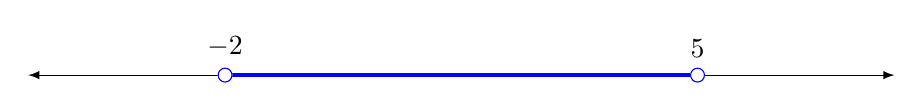
\begin{tikzpicture}
\draw[latex-latex] (-5.5,0) -- (5.5,0);
\draw[line width=1.5pt, color=blue] (-3,0) -- (3,0);
\filldraw[white](-3,0)circle[radius=2.5pt];
\draw[blue](-3,0)circle[radius=2.5pt];
\filldraw[white](3,0)circle[radius=2.5pt];
\draw[blue](3,0)circle[radius=2.5pt];
\node[at={(-3,3pt)},above]{$-2$};
\node[at={(3,3pt)},above]{$5$};
\end{tikzpicture}
\end{center}
Os círculos vazios $\circ$ indicam que os pontos finais não estão incluídos no intervalo.
\end{example}

Esteja avisado que o uso do símbolo $\infty$ é enganoso, pois sugere que o símbolo $\infty$ por si só tem um significado específico (ou, pior, que se refere a um número real). Isso não acontece - é apenas um símbolo que sugere a ilimitação do intervalo em questão. Uma maneira menos enganosa de escrever $[a, \infty)$, por exemplo, pode ser $[a, {\to})$ ou $\mathbb{R}^{\ge a}$; entretanto, $[a,\infty)$ é padrão, então é o que escreveremos.

\begin{exercise}
Para cada uma das ilustrações a seguir, encontre o intervalo que ela representa. Um círculo preenchido $\bullet$ indica que um ponto final está incluído no intervalo, enquanto um círculo vazio $\circ$ indica que um ponto final não está incluído no intervalo.

\begin{enumerate}[(a)]
\item
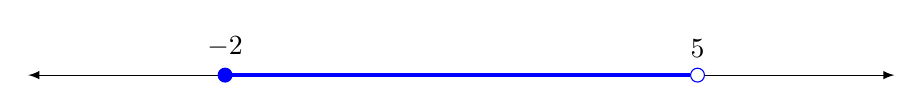
\begin{tikzpicture}
\draw[latex-latex] (-5.5,0) -- (5.5,0);
\draw[line width=1.5pt, color=blue] (-3,0) -- (3,0);
\filldraw[blue](-3,0)circle[radius=2.5pt];
\filldraw[white](3,0)circle[radius=2.5pt];
\draw[blue](3,0)circle[radius=2.5pt];
\node[at={(-3,3pt)},above]{$-2$};
\node[at={(3,3pt)},above]{$5$};
\end{tikzpicture}

\item
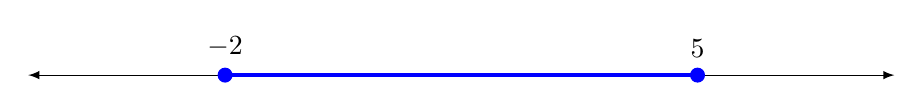
\begin{tikzpicture}
\draw[latex-latex] (-5.5,0) -- (5.5,0);
\draw[line width=1.5pt, color=blue] (-3,0) -- (3,0);
\filldraw[blue](-3,0)circle[radius=2.5pt];
\filldraw[blue](3,0)circle[radius=2.5pt];
\node[at={(-3,3pt)},above]{$-2$};
\node[at={(3,3pt)},above]{$5$};
\end{tikzpicture}


\item
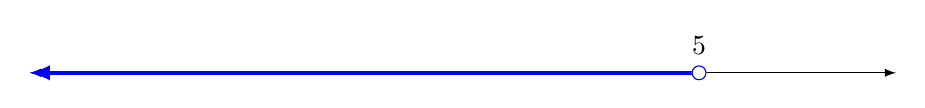
\begin{tikzpicture}
\draw[latex-latex] (-5.5,0) -- (5.5,0);
\draw[latex-, line width=1.5pt, color=blue] (-5.5,0) -- (3,0);
\filldraw[white](3,0)circle[radius=2.5pt];
\draw[blue](3,0)circle[radius=2.5pt];
\node[at={(3,3pt)},above]{$5$};
\end{tikzpicture}

\item 
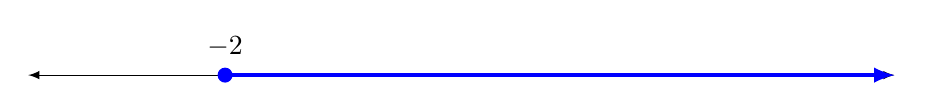
\begin{tikzpicture}
\draw[latex-latex] (-5.5,0) -- (5.5,0);
\draw[-latex, line width=1.5pt, color=blue] (-3,0) -- (5.5,0);
\filldraw[blue](-3,0)circle[radius=2.5pt];
\node[at={(-3,3pt)},above]{$-2$};
\end{tikzpicture}
\end{enumerate}
\end{exercise}

\subsection*{Subconjunto}

Muitas vezes acontece que tudo que também é elemento de um conjunto é elemento de outro conjunto. Por exemplo, todo número inteiro é um número racional; aquilo é
\[ \forall n \in \mathbb{Z},\, n \in \mathbb{Q} \]
Podemos dizer de forma mais concisa dizendo que $\mathbb{Z}$ é um \textit{subconjunto} de $\mathbb{Q}$.

\begin{definition}
\label{defSubset}
\index{subset}
Let $X$ be a set. A \textbf{subset} of $X$ is a set $U$ such that
\[ \forall a,\, (a \in U \Rightarrow a \in X) \]
Nós escrevemos $U \subseteq X$\nindex{subset}{$\subseteq$}{subset} \inlatex{subseteq}\lindexmmc{subseteq}{$\subseteq$} para a afirmação de que $U$ é um subconjunto de $X$.

Além disso, a notação $U \nsubseteq X$ \inlatex{nsubseteq}\lindexmmc{nsubseteq}{$\nsubseteq$} significa que $U$ não é um subconjunto de $X$, e a notação $U \subsetneqq X$ \ inlatex{subsetneqq}\lindexmmc{subsetneqq}{$\subsetneqq$} significa que $U$ é um \textbf{subconjunto próprio} de $X$, que é um subconjunto de $X$ que não é igual a $X$.
\end{definition}

\begin{strategy}[Provando uma contenção de subconjunto]
Para provar que um conjunto $U$ é um subconjunto de um conjunto $X$, basta pegar um elemento arbitrário $a \in U$ e provar que $a \in X$.
\end{strategy}

\begin{example}
Cada conjunto é um subconjunto de si mesmo --- isto é, $X \subseteq X$ para todos os conjuntos $X$. A prova disso é extremamente simples: devemos provar $\forall x \in X,\, x \in X$. Mas então isso é trivial: seja $x \in X$, então $x \in X$ por suposição. Feito!
\end{example}

\begin{example}
Seja $a,b,c,d \in \mathbb{R}$ with $a<c<d<b$. Então $[c,d] \subseteq (a,b)$. Na verdade, seja $x \in [c,d]$. Então $c \le x \le d$. Mas então
\[ a < c \le x \le d < b \quad \Rightarrow \quad a < x < b \]
para que $[c,d] \subseteq (a,b)$, como requerido.
\end{example}

\begin{exercise}
Seja $a,b,c,d \in \mathbb{R}$ com $a<b$ e $c<d$. Prove que $[a,b) \subseteq (c,d]$ se e somente se $a > c$ e $b \le d$.
\end{exercise}

\begin{example}
Os conjuntos de números de \Cref{chGettingStarted} estão relacionados pela seguinte cadeia de inclusões de subconjuntos.
\[ \mathbb{N} \subseteq \mathbb{Z} \subseteq \mathbb{Q} \subseteq \mathbb{R} \subseteq \mathbb{C} \]
\end{example}

A seguinte proposição prova uma propriedade de subconjunto conhecida como \textit{transitividade}---revisitaremos esta propriedade em \Cref{secRelations}.

\begin{proposition}
\label{propSubsetTransitive}
Seja $X,Y,Z$ conjuntos. Se $X \subseteq Y$ e $Y \subseteq Z$, then $X \subseteq Z$.
\end{proposition}

\begin{cproof}
Suponha que X⊆YX \subseteq Y e Y⊆ZY \subseteq Z. Precisamos provar X⊆ZX \subseteq Z.

Então vamos $a \in X$. Como $X \subseteq Y$, segue de \Cref{defSubset} que $a \in Y$; e como $Y \subseteq Z$, segue novamente de \Cref{defSubset} que $a \in Z$.

Portanto $X \subseteq Z$, conforme necessário.
\end{cproof}

\subsection*{Definindo igualdades}

Esta seção trata de definir conjuntos, comparar conjuntos e construir novos conjuntos a partir de antigos e, portanto, para progredir muito mais, primeiro precisamos estabelecer o que queremos dizer quando dizemos que dois conjuntos são \textit{iguais}.

\begin{discussion}
\label{dscSetEquality}
Sejam XX e YY conjuntos. O que deveria significar dizer que XX e YY são iguais? Tente fornecer uma definição precisa de igualdade de conjuntos antes de continuar lendo.
\end{discussion}

Existem diferentes noções possíveis de “semelhança” para conjuntos: poderíamos querer dizer que dois conjuntos XX e YY são iguais quando têm literalmente a mesma definição; ou podemos querer dizer que XX e YY são iguais quando contêm os mesmos objetos que elementos. Por exemplo, suponha que XX seja `o conjunto de todos os números naturais ímpares' e YY seja `o conjunto de todos os inteiros que são diferenças de quadrados perfeitos consecutivos' --- neste caso, a primeira destas caracterizações de igualdade pode nos levar a dizer X≠YX \ne Y, enquanto o segundo nos levaria a dizer X=YX = Y.

Claramente, teremos que declarar nossos termos em algum momento. E esse ponto é agora.

\begin{axiom}[Definir extensionalidade]
\label{axSetEquality}
\index{set equality}
\index{extensionality}
Sejam XX e YY conjuntos. Então $X=Y$ se e somente se $\forall a,\, (a \in X \Leftrightarrow a \in Y)$, ou equivalentemente, se $X \subseteq Y$ e $Y \subseteq X$.
\end{axiom}

Esta caracterização da igualdade de conjuntos sugere a seguinte estratégia para provar que dois conjuntos são iguais.

\begin{strategy}[Prova por dupla contenção]
Para provar que um conjunto XX é igual a um conjunto YY, basta:
\begin{itemize}
\item Prove $X \subseteq Y$, i.e.\ Seja $a \in X$ um elemento arbitrário e derive $a \in Y$; e então
\item Prove $X \supseteq Y$, i.e.\ Seja $a \in Y$ um elemento arbitrário e derive $a \in X$.
\end{itemize}
Frequentemente escrevemos `($\subseteq$)' e `($\supseteq$)' para indicar a direção da contenção que está sendo provada.
\end{strategy}

\begin{example}
\label{exPositiveNegativeSetBuilderNotation}
Provamos que $\{ x \in \mathbb{R} \mid x^2 \le 1 \} = [-1,1]$ por dupla contenção.
\begin{itemize}
\item ($\subseteq$) Seja $a \in \{ x \in \mathbb{R} \mid x^2 \le 1 \}$. Então $a \in \mathbb{R}$ e $a^2 \le 1$, para que $(1-a)(1+a) = 1-a^2 \ge 0$. Segue-se que ou:
\begin{itemize}
\item $1-a \ge 0$ e $1+a \ge 0$, nesse caso $a \le 1$ e $a \ge -1$, para que $a \in [-1,1]$.
\item $1-a \le 0$ e $1+a \le 0$, nesse caso $a \ge 1$ e $a \le -1$, o que é uma contradição já que $-1 < 1$.
\end{itemize}
Então devemos ter $a \in [-1,1]$, como requerido.

\item ($\supseteq$) Seja $a \in [-1,1]$. Então $-1 \le a \le 1$, então $|a| \le 1$, e desde então $a^2 = |a|^2 \le 1$, para que $a \in \{ x \in \mathbb{R} \mid x^2 \le 1 \}$, como requerido.
\end{itemize}
\end{example}

\begin{exercise}
Prove que {x∈R∣x2<x}=(0,1)\{ x \in \mathbb{R} \mid x^2 < x \} = (0,1).
\end{exercise}

O axioma da extensionalidade dos conjuntos tem como consequência que os conjuntos são independentes da ordem em que seus elementos aparecem na notação de lista e são independentes de quantas vezes um único elemento é escrito --- isto é, um elemento de um conjunto é apenas ` contado' uma vez, mesmo que apareça várias vezes na notação de lista. Isso é ilustrado no exercício a seguir.

\begin{exercise}
Prove por dupla contenção que {0,1}={1,0}\{ 0, 1 \} = \{ 1, 0 \} e {0,0}={0}\{ 0, 0 \} = \{ 0 \}.
\end{exercise}

\subsection*{Habitação e vazio}

Outro exemplo fundamental de conjunto é o \textit{conjunto vazio}, que é o conjunto sem elementos. Mas temos que ter um pouco de cuidado sobre como usamos a palavra `the', uma vez que ela implica \textit{unicidade}, e não sabemos (ainda) que dois conjuntos sem elementos são necessariamente iguais. Então, primeiro definiremos o que significa um conjunto vazio e depois mostraremos que existe exatamente um conjunto vazio.

\begin{definition}
\label{defInhabited}
\label{defEmptyProperty}
\index{empty set}
\index{set!empty}
\index{inhabited set}
\index{set!inhabited}
Um conjunto $X$ é \textbf{habitado} (ou \textbf{não vazio}) se possui pelo menos um elemento; caso contrário, está \textbf{vazio}.
\end{definition}

A afirmação de que $X$ é habitado é equivalente à fórmula lógica $\exists a,\, a \in X$, e a afirmação de que $X$ é vazio é equivalente à fórmula lógica $\neg \exists a,\ , um \em X$. Isto sugere a seguinte estratégia para provar que um conjunto é habitado ou que está vazio.

\begin{strategy}[Provando que um conjunto é habitado ou vazio]
Para provar que um conjunto $X$ é habitado, basta exibir um elemento. Para provar que um conjunto $X$ é vazio, suponha que $X$ seja habitado --- isto é, que exista algum elemento $a \in X$ --- e derive uma contradição.
\end{strategy}

Em outros textos, o termo \textit{nonempty} é mais comum que \textit{habitado}, mas há razões para preferir o último. Na verdade, a afirmação `$X$ não é vazio' se traduz mais diretamente em $\neg(\neg \exists a,\, a \in X)$, que tem uma dupla negativa desnecessária e sugere uma prova de habitação por contradição. Por esta razão, usamos o termo \textit{habitado} neste livro.

O vazio pode parecer uma condição trivial – e é – mas devido à sua canonicidade, ele surge em todos os lugares.

\begin{example}
O conjunto $\{ x \in \mathbb{R} \mid x^2 = 2 \}$ é habitado pois, por exemplo $\sqrt{2} \in \mathbb{R}$ e $\sqrt{2} ^2 = 2$. No entanto, o conjunto $\{ x \in \mathbb{Q} \mid x^2 = 2 \}$ está vazio, pois, se fosse habitado, então haveria um número racional $x$ tal que $x^2 = 2$, ao contrário de \Cref{propSqrt2IrrationalPreliminary}.
\end{example}

\begin{example}
Observamos em \Cref{exBracketN} que o conjunto $[0]$ está vazio; aqui está uma prova mais formal. Em direção a uma contradição, suponha que $[0]$ seja habitado. Então existe algum $k \in \mathbb{N}$ tal que $1 \le k \le 0$. Segue-se que $1 \le 0$, o que contradiz o fato de que $0<1$. Portanto, $[0]$ está vazio, afinal.
\end{example}

\begin{exercise}
Seja $a,b \in \mathbb{R}$. Prove que $[a,b]$ é vazio se e somente se $a > b$, e que $(a,b)$ é vazio se e somente se $a \ge b$.
\end{exercise}

O próximo exercício é um detalhe técnico lógico, que é contra-intuitivo pela mesma razão que torna o princípio da explosão (\Cref{axPrincipleOfExplosion}) difícil de compreender. Contudo, é extremamente útil para provar fatos sobre o conjunto vazio, como veremos em breve em \Cref{thmEmptySetIsUnique}.

\begin{exercise}
Seja $E$ um conjunto vazio e seja $p(x)$ um predicado com uma variável livre $x$ com domínio de discurso $E$. Mostre que a proposição $\forall x \in E,\, p(x)$ é verdadeira, e que a proposição $\exists x \in E,\, p(x)$ é falsa. O que significa a proposição $\forall x \in E,\, x \ne x$ em inglês? É verdade?
\hintlabel{exEverythingIsTrueOfElementsOfEmptySet}{%
Lembre-se do início de \Cref{secSets} que $\forall x \in X,\, p(x)$ é equivalente a $\forall x,\, (x \in X \Rightarrow p(x))$ e $\exists x \in X,\, p(x)$ é equivalente a $\exists x,\, (x \in X \wedge p(x))$. O que pode ser dito sobre o valor verdade de $x \in E$ quando $E$ está vazio?
}
\end{exercise}

Graças ao axioma da extensionalidade (\Cref{axSetEquality}), quaisquer dois conjuntos vazios devem ser iguais, uma vez que ambos contêm os mesmos elementos --- ou seja, nenhum elemento! Isso é formalizado no seguinte teorema.

\begin{theorem}
\label{thmEmptySetIsUnique}
Seja $E$ e $E'$ sejam conjuntos. Se $E$ e $E'$ são vazios, então $E=E'$.
\end{theorem}
\begin{proof}
Suponha que $E$ e $E'$ estejam vazios. A afirmação de que $E=E'$ é equivalente a
\[ (\forall a \in E,\, a \in E') \wedge (\forall a \in E',\, a \in E) \]
Mas $\forall a \in E,\, a \in E'$ e $\forall a \in E',\, a \in E$ são ambos verdadeiros por \Cref{exEverythingIsTrueOfElementsOfEmptySet} desde que $E$ e $E'$ sejam vazios. Então $E=E'$, como afirmado.
\end{proof}

Saber que existe um e apenas um conjunto vazio significa que podemos agora fazer a seguinte definição, sem nos preocupar se a palavra “o” é problemática.

\begin{definition}
\label{defEmptySet}
\nindex{O}{$\varnothing$}{empty set}
\index{empty set}
\index{set!empty}
The \textbf{conjunto vazio} (também conhecido como \textbf{conjunto nulo}) é o conjunto sem elementos e é denotado por $\varnothing$ \inlatex{varnothing}\lindexmmc{varnothing}{$\varnothing$}.
\end{definition}

Alguns autores escrevem $\{ \}$ em vez de $\varnothing$, já que $\{ \}$ é simplesmente o conjunto vazio expresso em notação de lista.

\begin{exercise}
\label{exEmptySetSubsetOfEverySet}
Seja $X$ um conjunto. Prove que $\varnothing \subseteq X$.
\end{exercise}

\subsection*{Conjuntos de Poder}

\begin{definition}
\label{defPowerSet}
\index{power set}
Se $X$ o conjunto. o \textbf{conjunto de potência} de $X$, escrito $\mathcal{P}(X)$\nindex{PX}{$\mathcal{P}(X)$}{conjunto de potência} \inlatex{mathcal\{ P\}}\lindexmmc{mathcal}{$\mathcal{A}, \mathcal{B}, \dots$}, é o conjunto de todos os subconjuntos de $X$.
\end{definition}

\begin{example}
Existem quatro subconjuntos de $\{ 1, 2 \}$, a saber
\[ \varnothing, \quad \{ 1 \}, \quad \{ 2 \}, \quad \{ 1, 2 \} \]
so $\mathcal{P}(X) = \{\varnothing, \{ 1 \}, \{ 2 \}, \{ 1, 2 \}\}$.
\end{example}

\begin{exercise}
Escreva os elementos de $\mathcal{P}(\{1, 2, 3\})$.
\end{exercise}

\begin{exercise}
Seja $X$ um conjunto. Mostre isso $\varnothing \in \mathcal{P}(X)$ e $X \in \mathcal{P}(X)$.
\end{exercise}

\begin{exercise}
Escreva os elementos de $\mathcal{P}(\varnothing)$, $\mathcal{P}(\mathcal{P}(\varnothing))$ e $\mathcal{P}(\mathcal{P}(\mathcal{P}(\varnothing)))$.
\end{exercise}

Conjuntos de potências costumam ser um ponto de confusão porque trazem a propriedade de ser um \textit{subconjunto} de um conjunto para a de ser um \textit{elemento} de outro, no sentido de que para todos os conjuntos $U$ e $X $ nós temos
\[ U \subseteq X \quad \Leftrightarrow \quad U \in \mathcal{P}(X) \]
Essa distinção parece fácil de entender, mas quando os conjuntos $U$ e $X$ são parecidos, é fácil cair em várias armadilhas. Aqui está um exemplo simples.

\begin{example}
É verdade que $\varnothing \subseteq \varnothing$, mas falso que $\varnothing \in \varnothing$. De fato,
\begin{itemizar}
\item $\varnothing \subseteq \varnothing$ significa $\forall x \in \varnothing,\, x \in \varnothing$; mas proposições da forma $\forall x \in \varnothing,\, p(x)$ são sempre verdadeiras, conforme discutido em \Cref{exEverythingIsTrueOfElementsOfEmptySet}.
\item O conjunto vazio não possui elementos; se $\varnothing \in \varnothing$ fosse verdade, isso significaria que $\varnothing$ tinha um elemento (esse elemento sendo $\varnothing$). Portanto, deve ser o caso de $\varnothing \not \in \varnothing$.
\end{itemize}
\end{example}

O exercício a seguir destina-se a ajudá-lo a superar possíveis tipos de confusão semelhantes por meio da prática. Tente pensar precisamente sobre quais são as definições envolvidas.

\begin{exercise}
Determine, com prova, se cada uma das afirmações a seguir é verdadeira ou não.
\begin{enumerate}[(a)]
\item $\mathcal{P}(\varnothing) \in \mathcal{P}(\mathcal{P}(\varnothing))$;
\item $\varnothing \in \{ \{ \varnothing \} \}$;
\item $\{ \varnothing \} \in \{ \{ \varnothing \} \}$;
\item $\mathcal{P}(\mathcal{P}(\varnothing)) \in \{ \varnothing, \{ \varnothing, \{ \varnothing \} \} \}$.
\end{enumerate}
Repita o exercício com todas as instâncias de `$\in$' substituídas por `$\subseteq$'.
\end{exercise}

\begin{tldr}{secSets}

\subsubsection*{Conjuntos e subconjuntos}

\begin{tldrlist}
\tldritem{defSet} Um \textit{set} é uma coleção de objetos (chamados \textit{elementos}) de um \textit{universo de discurso} fixo U\mathcal{U}; escrevemos x∈Xx \in X para significar que xx é um elemento do conjunto XX. Os conjuntos podem ser especificados (explícita ou implicitamente) listando seus elementos {x1,x2,…,xn,…}\{ x_1, x_2, \dots, x_n, \dots \}, ou usando \textit{notação set-builder} {x∈X meiop(x)}\{ x \in X \ meio p(x) \}.
\tldritem{defSubset} Um conjunto UU é um \textit{subconjunto} de um conjunto XX, escrito U⊆XU \subseteq X, se ∀a,(a∈U⇒a∈X)\forall a,\, (a \in U \Rightarrow a \in X). Para provar que U⊆XU \subseteq X, basta introduzir uma variável aa, assumir que a∈Ua \in U, e derivar a∈Xa \in X.
\tldritem{axSetEquality} Os conjuntos XX e YY são iguais se e somente se ∀a,(a∈X⇔a∈Y)\forall a,\, (a \in X \Leftrightarrow a \in Y). Para provar que X=YX = Y, basta provar separadamente que X⊆YX \subseteq Y e Y⊆XY \subseteq X --- este método é chamado \textit{dupla contenção}.
\end{tldrlist}

\subsubsection*{Habitação e vazio}

\begin{tldrlist}
\tldritem{defInhabited} Um conjunto XX é \textit{habitado} se tiver pelo menos um elemento; caso contrário, está \textit{vazio}.
\tldritem{thmEmptySetIsUnique} Existe um conjunto vazio único, denotado por ∅\varnothing or {}\{ \}.
\end{tldrlist}

\subsubsection*{Conjuntos de energia}
\begin{tldrlist}
\tldritem{defPowerSet} O \textit{conjunto de potências} de um conjunto XX é o conjunto de todos os subconjuntos de XX.
\end{tldrlist}
\end{tldr}
